\documentclass[aspectratio=169,xcolor=table]{beamer}
\usepackage{algorithm}
\usepackage{algpseudocode}
\usepackage[utf8]{inputenc}
\usepackage[T1]{fontenc}
\usepackage{lipsum, lmodern}
\usepackage{csquotes}
\usepackage{xcolor}
\usepackage[portuguese]{babel}

% ------------------------------------------------
% Tema e Configurações do Beamer
% ------------------------------------------------
\usetheme{DCC}

% Ajuste de espaçamento entre itens
\setbeamertemplate{itemize items}[circle]
\setbeamertemplate{itemize subitem}[circle]
\setlength{\itemsep}{0.8em}
\setlength{\parskip}{0.5em}

\graphicspath{{imgs/}{./imgs/}}

\author[Sena, Luis Felipe; Soares, Antoniel; Leahy, João]{%
  \textbf{Luis Felipe} \and \textbf{Antoniel Soares} \and \textbf{João Leahy}
}
\title{Análise de Interface: Telegram}
\subtitle{Aplicação de Conceitos de Interação Humano-Computador}
\institute{Universidade Federal da Bahia \\ Instituto de Computação}
\date{\today}

\begin{document}

%-------------------------------------------------
%  SLIDE DE TÍTULO
%-------------------------------------------------
\begin{frame}[plain,noframenumbering]
    \titlepage
\end{frame}

%-------------------------------------------------
%  SLIDE DE AGENDA
%-------------------------------------------------
\begin{frame}{Agenda}
    \tableofcontents
\end{frame}

\setlength{\parskip}{1em}

%=================================================
\section{Introdução}
%=================================================
\begin{frame}{Introdução}
    \begin{center}
        
\includegraphics[height=0.4\textheight]{telegram-logo.png}
    \end{center}
    \vspace{0.5em}
    \begin{itemize}
        \item \textbf{Interface Analisada:} Telegram (Aplicativo móvel)
        \item \textbf{Objetivo:} Aplicar conceitos de Interação Humano-Computador (IHC) para analisar a interface do Telegram, identificando aspectos positivos e oportunidades de melhoria.
    \end{itemize}
\end{frame}

%=================================================
\section{Conceitos de IHC Aplicados}
%=================================================
\begin{frame}{Conceitos de IHC Aplicados: Usabilidade}
    \begin{center}
        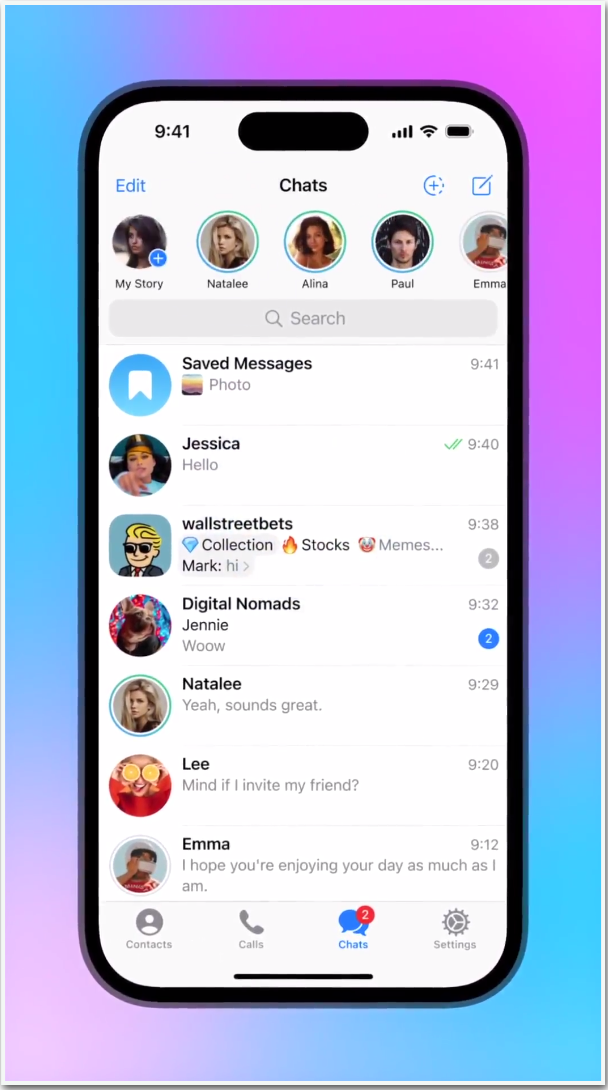
\includegraphics[height=0.4\textheight]{telegram-interface.jpg}
    \end{center}
    
    A facilidade com que os usuários conseguem utilizar o Telegram para atingir seus objetivos.
    
    \begin{itemize}
        \item \textbf{Exemplos no Telegram:} Interface intuitiva para envio de mensagens, criação de grupos e canais, busca de contatos e mídias.
    \end{itemize}
\end{frame}

\begin{frame}{Conceitos de IHC Aplicados: Acessibilidade}
    \begin{center}
        
\includegraphics[height=0.4\textheight]{acessibilidade.png}
    \end{center}
    
    Como o Telegram atende a usuários com diferentes capacidades e necessidades.
    
    \begin{itemize}
        \item \textbf{Exemplos no Telegram:} Opções de personalização de tamanho de fonte, temas com contraste ajustável, suporte a leitores de tela (parcial).
        \item \textbf{Oportunidade:} Melhorar a navegação e descrição de elementos para leitores de tela.
    \end{itemize}
\end{frame}

\begin{frame}{Conceitos de IHC Aplicados: Design Centrado no Usuário}    
    Se a interface foi projetada considerando as necessidades, expectativas e limitações dos usuários finais.
    
    \begin{itemize}
        \item \textbf{Exemplos no Telegram:} Foco na velocidade e segurança, armazenamento em nuvem, múltiplos dispositivos, funcionalidades como pastas e chats arquivados.
    \end{itemize}
\end{frame}

\begin{frame}{Conceitos de IHC Aplicados: Eficiência e Intuitividade}
    \begin{center}
        
\includegraphics[height=0.4\textheight]{telegram-chat.jpg}
    \end{center}
    
    O quão rapidamente os usuários conseguem realizar tarefas e se a interface é intuitiva.
    
    \begin{itemize}
        \item \textbf{Exemplos no Telegram:} Atalhos para ações comuns (responder, encaminhar), organização de conversas, pré-visualização de links e mídias.
        \item \textbf{Intuitividade:} Ícones claros e fluxos de interação geralmente diretos.
    \end{itemize}
\end{frame}

\begin{frame}{Conceitos de IHC Aplicados: Estética e Percepção}
    \begin{center}
        
\includegraphics[height=0.4\textheight]{telegram-temas.jpg}
    \end{center}
    
    Como o design visual influencia a experiência do usuário e a percepção da interface.
    
    \begin{itemize}
        \item \textbf{Exemplos no Telegram:} Design limpo e personalizável (temas, planos de fundo), uso consistente de cores e tipografia. Animações sutis que melhoram a experiência sem sobrecarregar.
    \end{itemize}
\end{frame}

%=================================================
\section{Pontos Fortes e Fracos}
%=================================================
\begin{frame}{Pontos Fortes do Telegram}
    \begin{itemize}
        \item \textbf{Velocidade e Leveza:} Resposta rápida da interface.
        \item \textbf{Personalização:} Ampla gama de temas e ajustes visuais.
        \item \textbf{Funcionalidades Avançadas:} Bots, canais, supergrupos, pastas.
        \item \textbf{Multiplataforma Sincronizada:} Uso transparente em diversos dispositivos.
        \item \textbf{Armazenamento em Nuvem:} Facilidade de acesso a mídias e histórico.
    \end{itemize}
\end{frame}

\begin{frame}{Pontos Fracos do Telegram}
    \begin{itemize}
        \item \textbf{Descoberta de Funcionalidades:} Algumas funcionalidades avançadas podem ser difíceis de encontrar para novos usuários.
        \item \textbf{Acessibilidade:} Pode haver melhorias para usuários com deficiências visuais severas em certas áreas.
        \item \textbf{Curva de Aprendizagem Inicial:} A quantidade de recursos pode ser intimidadora para alguns usuários inicialmente.
    \end{itemize}
\end{frame}

%=================================================
\section{Propostas de Melhoria}
%=================================================
\begin{frame}{Propostas de Melhoria: Tutorial Interativo Opcional}
    \begin{itemize}
        \item \textbf{Descrição:} Um tutorial guiado e opcional que apresente as principais funcionalidades e configurações do Telegram de forma interativa, especialmente para novos usuários.
        \item \textbf{Justificativa (IHC):} Melhora a \textbf{Eficiência e Intuitividade} para novos usuários, reduzindo a curva de aprendizado e auxiliando na descoberta de recursos (aborda um Ponto Fraco).
    \end{itemize}
\end{frame}

\begin{frame}{Propostas de Melhoria: Central de Acessibilidade Aprimorada}
    \begin{itemize}
        \item \textbf{Descrição:} Uma seção dedicada e mais robusta para configurações de acessibilidade, com pré-visualizações claras das alterações e talvez perfis de acessibilidade pré-definidos.
        \item \textbf{Justificativa (IHC):} Fortalece a \textbf{Acessibilidade}, tornando mais fácil para usuários com diferentes necessidades configurarem o aplicativo (aborda um Ponto Fraco).
    \end{itemize}
\end{frame}

%=================================================
\section{Conclusão}
%=================================================
\begin{frame}{Conclusão}
    \begin{center}
        
\includegraphics[height=0.4\textheight]{telegram-logo.png}
    \end{center}
    
    O Telegram apresenta uma interface robusta, com fortes características de usabilidade, eficiência e design centrado no usuário. As propostas de melhoria focam em aprimorar a experiência inicial e a acessibilidade, tornando o aplicativo ainda mais inclusivo e fácil de usar para um espectro mais amplo de usuários.
\end{frame}

%=================================================
\section{Perguntas e Comentários}
%=================================================
\begin{frame}{Perguntas e Comentários}
    \begin{center}
        \Huge Obrigado!
    \end{center}
\end{frame}

\end{document}
